\chapter{Methodik}

Nachfolgdend wird die vollständige Vorgehensweise der Versuchsdurchführung erklärt.
Dazu ist es notwendig eine Methodik zu definieren.

In der Browserforensik ist eine definierte Methodik notwendig, um die Komplexität moderner Browser zu bewältigen. Sie bildet bildet eine wissenschaftliche Basis für den durchgeführten Versuch sowie einen Leitfaden für Ermittler bei zukünftigen Untersuchungen. \cite{Aggarwal.2010, Izzati.2022, Horsman.2019}	
Ein oft verwendetes Vorgehensmodell in der Computer Forensik ist das "Generic Model Computer Forensics Investigations", kurz GCFIM. \cite{Yusoff.2011}
Ähnlich zum "abschnittsbasierter Verlauf einer forensischen Untersuchung" des Bundesamt für Sicherheit in der Informationstechnik ist es in Phasen mit definierten Abläufen gegliedert.
% https://www.bsi.bund.de/SharedDocs/Downloads/DE/BSI/Cyber-Sicherheit/Themen/Leitfaden_IT-Forensik.pdf?__blob=publicationFile&v=2

Izzati et al. haben diese Phasen auf Browserforensik abgebildet: \cite{Izzati.2022}
\begin{itemize}
	\item Vorbereitung: Versuchsplanung und Konfiguration der Versuchsumgebung.
	\item Datensammlung: Speicherabbilder identifizieren und während des Browsing Szenarios erstellen. 
	\item Datenanalyse: Suche nach Browsing Artefakten in gesammelten Daten.
	\item Dokumentation: Vorgehensweise und gefundene Artefakte dokumentieren.
\end{itemize}

Die Dokumentationsphase entspricht in dieser Arbeit Kapitel "Vergleich der Browser" (TODO!). Die Methodik der anderen Phasen wird nachfolgend beschrieben.

\section{Vorbereitung}

In der Vorbereitungsphase wird der durchgeführte Versuch geplant sowie die Versuchsumgebung konfiguriert. \cite{Izzati.2022} Versuchsplanung zählt die Auswahl von Browsern und Tools sowie die Definition eines durchzuführenden Browsing-Szenarios. Die Konfiguration der Versuchsumgebung umfasst die Installation und Konfiguration der notwendigen Software und Hardware.

\subsection{Browserauswahl}

Für diese Arbeit dazu entschieden: zwei weit verbreitete Brower verwenden + zwei Browser mit verstärkem Schutz der Privatsphäre.

Dazu: Google Chrome und Mozilla Firefox ausgewählt.

Weiterhin werden zwei Browser mit verstärkem Schutz der Privatsphäre ausgewählt.
Basierend auf Chromium wird der Browser "Brave" gewählt.
Für Firefox wird der Tor-Browser gewählt, eine modifizierte Version von Firefox.

\subsubsection*{Firefox}

Der Browser Mozilla Firefox, kurz Firefox, ist ein open-source Webbrowser der gemeinnützigen Organisation Mozilla. 
Firefox hat die Funktion des "privaten Modus". Diese ermöglicht es, ohne Speicherung von Verlaufsdaten und Cookies zu im Internet zu Browsen.
Laut Firefox wird mit dem privaten Modus vor dem "Lokalen Angreifer" geschützt, wie er in Kapitel X (TODO!) definiert ist, jedoch nicht vor dem Webangreifer.
Es wird ausdrücklich darauf hingewiesen, dass die besuchten Webseiten und Ihr Internetanbieter (ISP)  weiterhin anhand Ihrer IP-Adresse Informationen über die von Ihnen besuchten Seiten sammeln, selbst wenn Sie nicht angemeldet sind. 
% https://www.mozilla.org/de/firefox/
% https://www.mozilla.org/de/about/history/
Für diesen Versuch: Firefox Version 112.0.2 (64 Bit)

\subsubsection*{Tor}

Der Tor Browser, früher Tor Browser Bundle, ist ein auf Firefox basierender Webbrowser, der das Tor-Netzwerk nutzt.
Der Tor Browser wirbt im Gegensatz zu Firefox mit Schutzmaßnahmen gegen Webangreifer.
Internetdienstanbieter können Internetaktivitäten aufgrund Natur des Tor-Netzwerks nicht verfolgen.
Der Tor Browser wirbt mit folgendem Schutzmaßnahmen gegen lokalen Angreifer:
- Tor Browser does not keep any browsing history. Cookies are only valid for a single session (until Tor Browser is exited or a New Identity is requested).
Zusätzliche Funktion: "Neue Identität"
\begin{figure}[h!]
	\resizebox{\linewidth}{!}{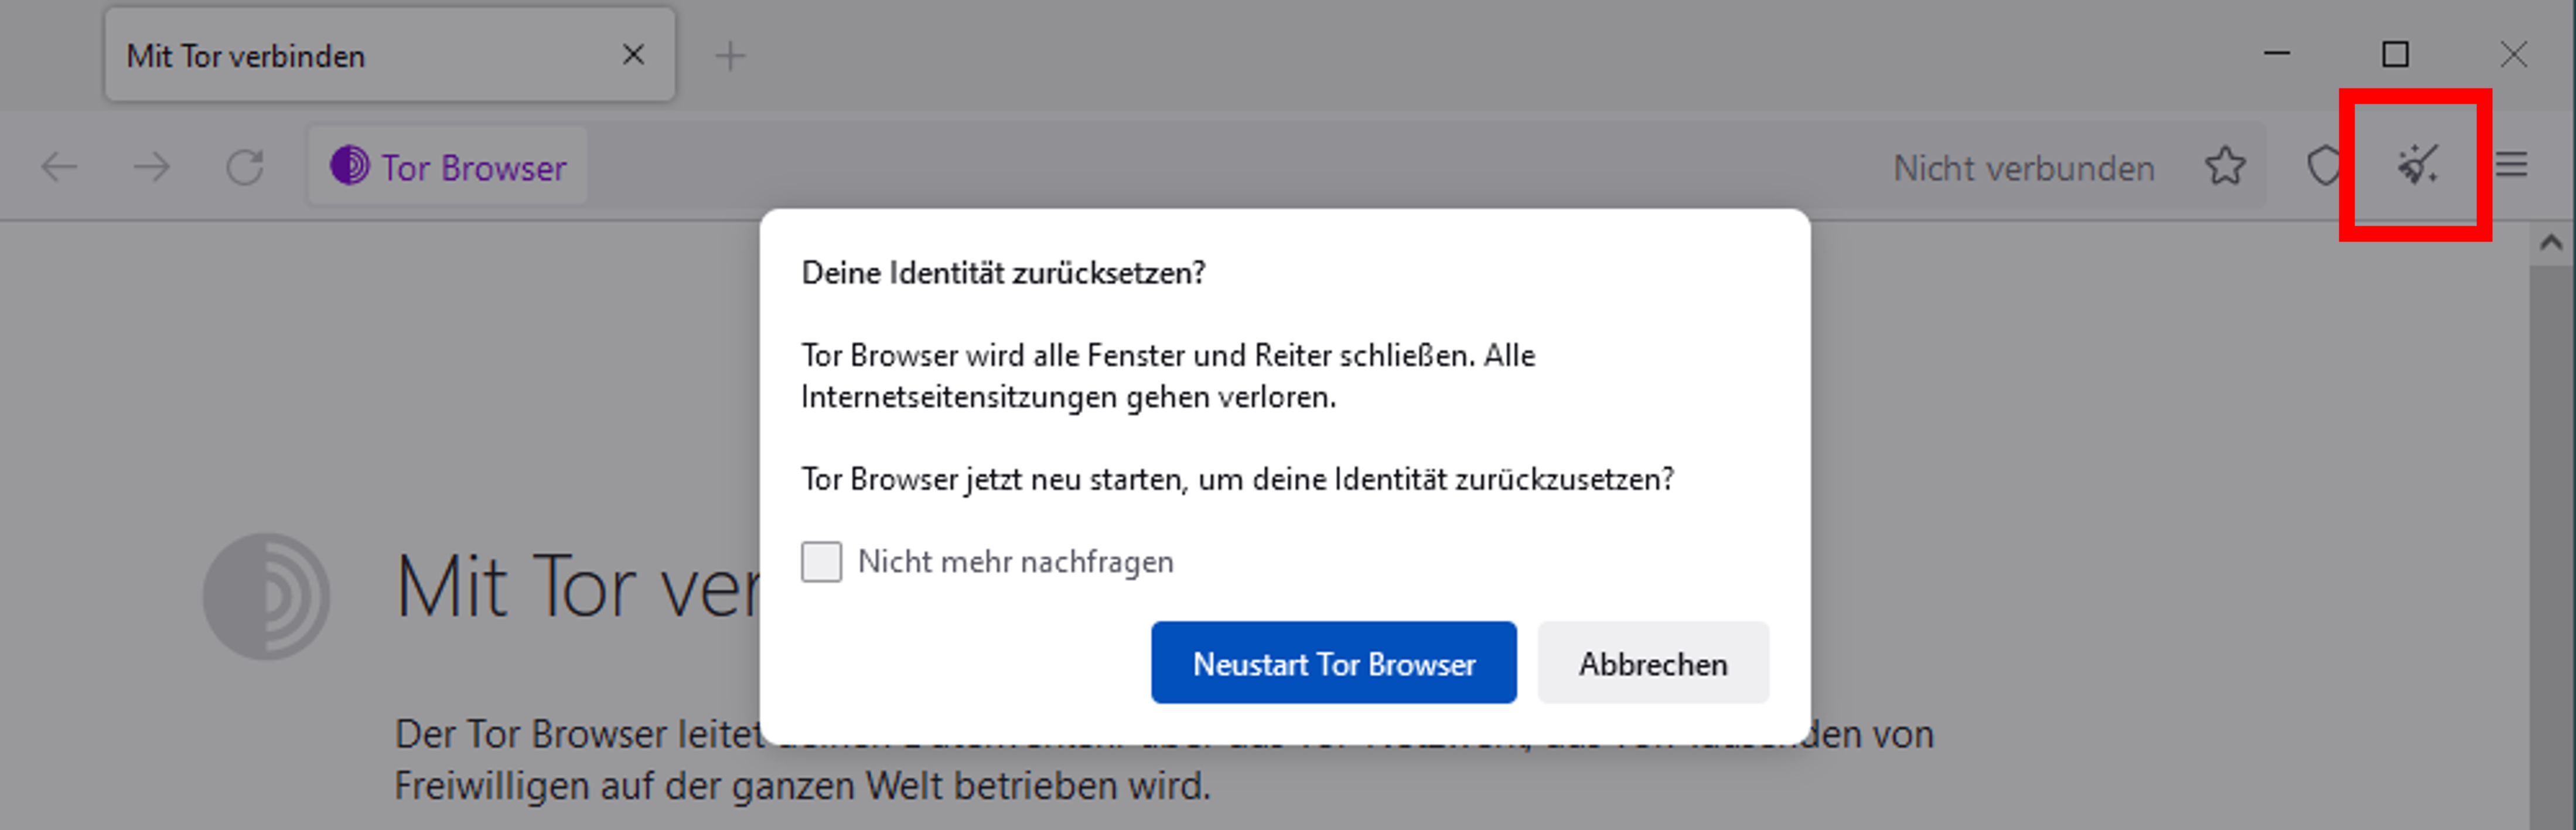
\includegraphics{bilder/tor-new-identity.png}}
%	\label{...}
	\caption{Tabelle mit wiederherstellbaren Dateien: Logfile 1 vs. Logfile 2}
\end{figure}
Die Funktion "Neue Identität" im Tor Browser ermöglicht es, alle aktuellen Tabs und Fenster zu schließen, sämtliche private Informationen wie Cookies und Verlauf zu löschen und für alle Verbindungen neue Relays zu verwenden.
Für diesen Versuch: Tor Version 12.0.4 (64 Bit)

\subsubsection*{Chrome}

\subsubsection*{Brave}

\subsection{Browsing Szenario}

% > Image als Hex: \cite{Ohana.2013}

Für Versuch definiert, mit welchen Daten der Rechner kontaminiert werden soll.
Im Falle der Browser-Forensik werden eine Reihe von Aktivitäten definiert, die für jeden zu untersuchenden Browser durchgeführt werden, das sog. "Browsing Szenario".

- Ziel: PB Artefakte, die ausschließlich in Browsing-Szenario vorkommen, bspw. "twitter" oder "facebook" bereits in vielen Windows-Standardanwendungen enthalten.
- (TODO: Literatur)

Folgende Schritte werden in jedem Browser durchgeführt: 

\begin{enumerate}
\item  www.google.com aufrufen
	\begin{enumerate}[label*=\arabic*.]
	\item Alle Cookies akzeptieren 
	\item Google-Suche nach "pfaffenhofen"
	\end{enumerate}
\item www.google.com aufrufen
	\begin{enumerate}[label*=\arabic*.]
	\item Cookies alle akzeptieren 
	\item Google-Suche nach "nanoradar" 
	\end{enumerate}
\item www.google.com aufrufen
	\begin{enumerate}[label*=\arabic*.]
	\item Cookies alle akzeptieren 
	\item Google-Suche nach "mallofamerica"
	\item Auf Suchergebnis "mallofamerica.com" klicken
	\end{enumerate}
\item www.google.com aufrufen
	\begin{enumerate}[label*=\arabic*.]
	\item Cookies alle akzeptieren 
	\item Google-Suche nach "mooserliesl"
	\item Auf Suchergebnis "mooserliesl.de" klicken
	\end{enumerate}
\item "www.unitree.com" über URL-Leiste öffnen
\item "www.donaukurier.de" über URL-Leiste öffnen
	\begin{enumerate}[label*=\arabic*.]
	\item Donaukurier Logo in neuem Tab öffnen
	\end{enumerate}
\item "mail.google.com" über URL-Leiste öffnen
	\begin{enumerate}[label*=\arabic*.]
	\item Mit google Account anmelden: 
			\begin{enumerate}[label*=\arabic*.]
			\item E-Mail = "computerforensikvl@gmail.com"
			\item Passwort = "Vorlesung23!"
			\end{enumerate}
	\item Neue E-Mail schreiben:
			\begin{enumerate}[label*=\arabic*.]
			\item Empfänger: "cas0597@thi.de" und "chs3702@thi.de"
			\item Betreff: "Betrefftext"
			\item Mailinhalt: "Mailinhalt"
			\end{enumerate}			
	\end{enumerate}
\end{enumerate}

Aus diesem Browsing-Szenario lassen sich die in Tabelle X dargestellten "private Browsing Artefakte", kurz PB Artefakte ableiten. Dabei handelt es sich dabei um Strings oder reguläre Ausdrücke, die eindeutig einem Schritt im Browsing-Szenario zugeordnet werden können.

\begin{table}[h!]
\centering
\begin{tabular}{|c|l|c|}
\hline
\textbf{Kategorie}           & \multicolumn{1}{c|}{\textbf{Private Browsing Artefakt}}                                      & \textbf{\begin{tabular}[c]{@{}c@{}}Schritt im\\  Browsing Szenario\end{tabular}} \\ \hline
\multirow{4}{*}{Suchbegriff} & "pfaffenhofen"                                                                               & 1.2                                                                              \\ \cline{2-3} 
                             & "nanoradar"                                                                                  & 2.2                                                                              \\ \cline{2-3} 
                             & "mallofamerica"                                                                              & 3.2                                                                              \\ \cline{2-3} 
                             & "mooserliesl"                                                                                & 4.2                                                                              \\ \hline
\multirow{4}{*}{URL}         & "mooserliesl.de"                                                                             & 3.3                                                                              \\ \cline{2-3} 
                             & "mallofamerica.com"                                                                          & 4.3                                                                              \\ \cline{2-3} 
                             & "unitree.com"                                                                                & 5.                                                                               \\ \cline{2-3} 
                             & "donaukurier.de"                                                                             & 6.                                                                               \\ \hline
Bild                         & \begin{tabular}[c]{@{}l@{}}0x89 0x50 0x4E 0x47 ...\\ (PNG als Hexadezimalwerte)\end{tabular} & 6.1                                                                              \\ \hline
\multirow{4}{*}{E-Mail}      & "computerforensikvl@gmail.com"                                                               & 7.1.1                                                                            \\ \cline{2-3} 
                             & "Vorlesung23!"                                                                               & 7.1.2                                                                            \\ \cline{2-3} 
                             & "cas0597@thi.de"                                                                             & 7.2.1                                                                            \\ \cline{2-3} 
                             & "chs3702@thi.de"                                                                             & 7.2.1                                                                            \\ \hline
\end{tabular}
\end{table}


\subsection*{VM Konfiguration}

Best Practice in Browser Forensik: Versuche sowie Analysen in virtualisierter Umgebung durchführen. (TODO: Quellen)
- Dadurch Reproduzierbarkeit der Ergebnisse sichergestellt
- Keine Vermischung der PB Artefakte, wenn gleicher Rechner verwendet
- Keine Vermischung der Versuchsumgebung mit der Analyseumgebung
- Ergebnisse sind transportabel -> Zustände von Virtuellen Maschinen exportierbar
- Deshalb oft in Literatur empfohlen

Als Virtualisierungssoftware für Versuch verwendet: Kostenlose Oracle VirtualBox VM, Version 7.0.8 r156879 (Qt5.15.2)

Pro Browser wird eine VM erstellt, auf der Browsing Szenario durchgeführt wird. Alle VMs basieren auf gleicher OVA, deren Konfiguration in Tabelle X dargestellt ist.

\begin{table}[h!]
\centering
\begin{tabular}{|l|l|}
\hline
\textbf{Betriebssystem}         & Windows 10 Pro, 64 Bit, Build: 19045.2006                                  \\ \hline
\textbf{Festplatte}             & 30 GB, VDI-Format, kein SSD Laufwerk                                       \\ \hline
\textbf{RAM}                    & 6 GB                                                                       \\ \hline
\textbf{Netzwerk}               & Netzwerkbrücke                                                             \\ \hline
\textbf{Verbindung zu Host-PC}  & Gemeinsamer Ordner                                                         \\ \hline
\textbf{Installierte Programme} & \begin{tabular}[c]{@{}l@{}}Process Monitor (Version 3.93)\\ Process Explorer (Version 17.04)\end{tabular} \\ \hline
\end{tabular}
\end{table}

Um Programme auf VM zu installieren: Gemeinsamer Order zwischen VM und Rechner eingerichtet, auf dem VM läuft. Ordner wird in VM als Netzwerklaufwerk angezeigt
Grund: VM erst mit Beginn von Browsing Szenario mit Netzwerk und Internet verbinden. Deshalb: Programme mussten auf Rechner auf dem VM läuft heruntergeladen werden und über gemeinsamen Order auf VM transportiert werden.

Weiterhin wurden zwei Werkzeuge der Sysinternal-Abteilung von Microsoft installiert: "Process Monitor", zur Aufzeichnung aller Prozessaktivitäten sowie "Process Explorer", der die Funktionen des Windows Task Managers erweitert. 
% https://learn.microsoft.com/de-de/sysinternals/downloads/procmon
Für diesen Versuch verwendet: Version 3.93
% https://learn.microsoft.com/de-de/sysinternals/downloads/process-explorer
Für diesen Versuch verwendet: Version 17.04

\subsubsection*{Browserinstallation}
Zunächst Browser installiert. Folgende Installationsverzeichnisse verwendet:
\begin{enumerate}
\item[\textbf{Firefox}] \texttt{C:$\backslash$Program Files$\backslash$Mozilla Firefox$\backslash$firefox.exe}
\item[\textbf{Tor}] \texttt{C:$\backslash$Program Files$\backslash$Tor Browser$\backslash$Browser$\backslash$firefox.exe}
\item[\textbf{Chrome}] ***TODO!***
\item[\textbf{Brave}] ***TODO!***
\end{enumerate}

\subsection{Analysewerkzeuge}

Neben Konfiguration der VM muss Analyseumgebung vorbereitet werden.
Als Analyseumgebung dient der Rechner, auf dem die VM läuft.
Spezifikationen: *** TODO ***
Dazu: Diverse Tools zur Analyse installieren

\subsubsection*{Autopsy}
Wie im nächsten Kapitel X (TODO!) beschrieben, müssen Festplattenabbilder untersucht werden.
Dazu wird in der Literatur das Tool "Autopsy" empfohlen.

Autopsy ist ein Open-Source-Digital-Forensik-Tool, das auf der Sleuthkit-Bibliothek basiert. 
Sleuthkit ist eine Sammlung von Open-Source-Tools für die forensische Analyse von Dateisystemen. Es bietet Funktionen zum Lesen, Analysieren und Wiederherstellen von Daten aus verschiedenen Dateisystemen. 
Autopsy baut auf der Funktionalität von Sleuthkit auf und bietet eine grafische Benutzeroberfläche für die forensische Analyse. 
Wurde hauptsächlich in Java geschrieben.
Es erweitert die Funktionalität von Sleuthkit, indem es zusätzliche Tools, Plug-Ins und Automatisierungsfunktionen bereitstellt, um den forensischen Untersuchungsprozess zu unterstützen.
 
Für diesen Versuch verwendet: Version 4.20.0

\subsubsection*{Volatility}
Neben der Analyse von Festplattenabbildern müssen gemäß Kapitel X Abbilder des Arbeitsspeichers unteruscht werden. Dazu wird das in der Literatur empfohlene Tool "Volatility" verwendet.
Das Volatility Memory Forensics Framework ist ein Open-Source-Tool, das für die forensische Analyse von Arbeitsspeicherabbildern verwendet wird. Es ist speziell darauf ausgerichtet, Informationen und Artefakte aus dem physischen oder virtuellen Arbeitsspeicher eines Computers zu extrahieren.
Geschrieben in Python, frei auf GitHub verfügbar:	
%Version: Volatility3, Version 2.4.1 (aktuellster Release)
Für diesen Versuch verwendet: "Volatility3"
= vollständige Neuschreibung des Volatility Memory Forensics Frameworks, die im Jahr 2020 veröffentlicht wurde. 
%Behebt technische und Performanceprobleme der vorherigen Version.
%Oft beworbender Vorteil von Volatility3: kein "Profile" mehr notwendig. Volatility3 erstellt Symboltabellen für Windows-Speicherabbilder basierend auf dem Speicherabbild selbst.
%Dabei handelt es sich um ein Konfigurationseinstellung, welche die Speicherstruktur und die Verhaltensweisen des Betriebssystems definiert.
	% https://volatility3.readthedocs.io/en/latest/vol2to3.html
	% https://www.volatilityfoundation.org/
	% https://github.com/volatilityfoundation/volatility3
Volatility basiert auf Plugins, welche spezifische Funktionen und Analysen für verschiedene Aspekte des Systems bereitstellen. Für diesen Versuch werden folgende Plugins verwendet. 
\begin{itemize}
\item pslist	
\item yarascan		
\item memmap	 	
\item filescan
\item svcscan
\end{itemize}
Genaue Beschreibung der PlugIns und deren Zusammenhang: Siehe Analysephase in Kapitel X (TODO!).		


\subsection*{Übersicht verwendete Software}

Tabelle X listet zusammenfassend alle in diesem Versuch verwendeten Software-Programme, deren Zweck sowie Version auf.

Neben den Programmen zur Analyse der Speicherabbilder: diverse zusätzliche unterstützende Tools zur vollständigen Analyse benötigt, diese werden nicht genauer beschrieben.
- Nur in Tabelle aufgenommen

\begin{table}[]
\resizebox{\linewidth}{!}{
\begin{tabular}{|l|l|l|}
\hline
\multicolumn{1}{|c|}{\textbf{Software}} & \multicolumn{1}{c|}{\textbf{Zweck}}                                              & \multicolumn{1}{c|}{\textbf{Version}} \\ \hline
Oracle VirtualBox                       & Virtualisierung                                                                  & 7.0.8 r156879                         \\ \hline
Windows 10 Pro                          & VM Betriebssystem                                                                & Build: 19045.2006                     \\ \hline
Process Monitor                         & Aufzeichnung Prozessaktivitäten                                                  & 3.93                                  \\ \hline
Process Explorer                        & Darstellung der Eigenschaften aktueller Prozesse                                 & 17.04                                 \\ \hline
Autopsy                                 & Analyse Festplattenabbilder                                                      & 4.20.0                                \\ \hline
Volatiltiy                              & Analyse RAM-Abbilder                                                             & Volatility3 Version 2.4.1             \\ \hline
HxD                                     & Analyse Binärdateien in hexadezimaler und ASCII-Darstellung                      & 2.5.0.0                               \\ \hline
Notepad++                               & Analyse strukturierter Dateiformate, z.B. JSON, XML                              & 8.4.5                                 \\ \hline
Registry Explorer                       & Grafischer Oberfläche zur Untersuchung von Windows-Registry Hives                & 2.0.0.0                               \\ \hline
DB Browser for SQLite                   & Grafische Oberfläche zur Verwaltung und Untersuchung von SQLite-Datenbanken      & 3.12.2                                \\ \hline
sqldiff.exe                             & Befehlszeilen-Programm zur Anzeige von Unterschieden zwischen SQLite-Datenbanken & 3.42.0                                \\ \hline
ChromeCacheView                         & Einlesen von Chrome Cache-Dateien und visuelle Aufbereitung des Inhalts          & 2.46                                  \\ \hline
MZCacheView                             & Einlesen von Firefox Cache-Dateien und visuelle Aufbereitung des Inhalts         & 2.21                                  \\ \hline
FirefoxCache2                           & Erweitert MZCacheView, um Firefox "index"-Cachedatei zu analysieren              & Commit b50ab4f                        \\ \hline
dejsonlz4                               & Dekomprimierung von .jsonlz4-Dateien                                             & Commit c4305b8                        \\ \hline
\end{tabular}
}
\end{table}



\section{Datensammlung}

*** TODO: Schreiben, dass für diesen Versuch auch VM-Snapshots zu bestimmten Zeitpunkten aufgetaut werden können ***

In der Phase der Datensammlung werden alle potenziellen Beweismittel identifiziert, gesammelt. Ziel ist es, die Daten in einem Format zu sammeln, in dem sie in der nächsten Phase analysiert werden können. \cite{Izzati.2022}

Für diesen Versuch umfasst dies die Durchführung des Browsing Szenarios sowie die Sammlung von Ressoucen, die potentielle private Browsing Artefakte enthalten.

\subsection*{Process Monitor Logfiles}

Um das Verhalten von privaten Browsingmodi möglichst vollständig zu untersuchen, schlagen Fayyad-Kazan et al. \cite{Fayyad.2021} vor, alle Aktivitäten des Browsers während Browsing-Szenarios aufzeichnen.
Dazu werden mithilfe des Tools "Process Monitor" alle Prozess-Aktivitäten aufgezeichnet 
und als "Process Monitor Logfile" (PML) oder CSV-Datei gespeichert. \cite{Fayyad.2021, Rochmadi.2017}
Die PML-Dateien werden dabei mithilfe des gemeinsamen Ordners auf den den Analyserechner transportiert.

\subsection*{Speicherabbilder}
Eine der Hauptaufgaben eines Computer-Forensischen-Ermittlers ist die Erstellung und Analyse von Speicherabbildern, direkte Kopien der Daten auf den Speichermedien des untersuchten Rechners. \cite{Hassan.2019}
Im Falle der Browser Forensik werden in der Literatur zwei Arten von Speichermedien untersucht: Festplatten und der Arbeitsspeicher.

\paragraph*{Festplatten-Image}
Da in diesem Versuch die Festplatten virtualisiert wurden, wird ein Festplatten-Abbild aus einem sogenannten "VM-Snapshot" gewonnen, eine Momentaufnahme einer virtuellen Maschine.  % https://docs.oracle.com/en/virtualization/virtualbox/6.0/user/snapshots.html
Bei Oracle VirutalBox kann eine VM Snapshot über die grafische Oberfläche durchgeführt werden.
Durch den Snapshot wird ein "Virtual Disk Image", eine VDI-Datei, im Snapshot-Ordner der VM erzeugt. Diese Laufwerksdatei enthält nur differentielle Daten zum vorherigen Snapshot.
Um aus den differentiellen Daten ein vollständiges Festplatten-Image zu erzeugen muss ein "vollständiger Klon" des Snapshots erstellt werden. Die VDI-Datei der geklonten VM enthält alle Festplatten-Daten zum Zeitpunkt des durchgeführten Snapshots.

Da Autopsy nicht das VDI-Format unterstützt, müssen die Laufwerksdateien der geklonten Snapshots in ein das generische Image-Format (.img) umgewandelt werden.
Durch Nutzung des VirtualBox Befehlszeilen-Tool "vboxmanage" wird mit dem Befehl \texttt{vboxmanage clonehd <VDI\_File>.vdi <IMG\_File>.img --format raw} die VDI-Datei ein eine IMG-Datei umgewandelt.

*** TODO: Hier Einlesen der Festplatten-Images => Zeitaufwändig! ***

\paragraph*{RAM-Dump}

Ein sogenannter "RAM-Dump" erfasst den genauen Zustand des Arbeitsspeichers, einschließlich der im Speicher befindlichen Daten, Programme und Prozesse.
% https://kollee.github.io/posts/memory-forensics-of-a-virtualbox-vm/
VirtualBox empfiehlt, Abbilder des Arbeitsspeichers ebenfalls über das "vboxmanage" Befehlszeilen-Tool durchzuführen.
Im Unterschied zu Festplatten-Images können RAM-Dumps mit dem Tool nur in angeschaltetem Zustand der virtellen Maschine durchgeführt werden. 
Dazu wird folgender Befehl ausgeführt: \texttt{vboxmanage debugvm <VM Name> dumpvmcore --filename "<RAM Dump Dateiname>.elf}. RAM-Dumps im .elf Format können direkt vom Analysetool Volatility eingelesen werden.		

\paragraph*{Zeitpunkte zur Datensammlung}
Wichtig für die qualität der Versuchsergebnisse ist das Festlegen der Zeitpunkte im Browsing Szenario zum Sammeln der Daten.
Dieses Thema wird in der Literatur kaum thematisiert. Die Autoren wählen die Zeitpunkte meist ohne Begründung.

Dieses Problem haben Muir, Leimich und Buchanan erkannt und Zeitpunkte zur Datensammlung vorgeschlagen, um das Browserverhalten während des Browsing-Szenarios vollständig zu überwachen und zu analysieren. Wie in Abbildung X (TODO!) dargestellt, wurde sich an diesen Zeitpunkten für diesen Versuch orientiert.
\begin{figure}[h!]
	\centering
	\small
	\centerline{\resizebox{\linewidth}{!}{\input{bilder/datensammlung-zeitpunkte-Latex.pdf_tex}}}
	\caption{Datensammlung Zeitpunkte}
	\label{fig:jes}
\end{figure}
Nach der Browser-Installation, vor Beginn des Browsing-Szenarios wird der erste RAM-Dump sowie der erste VM-Snapshot erstellt.
Diese Speicherabbilder dienen als Benchmark für die Analyse, da in diesen Speicherabbildern kein PB Artefakt gefunden werden darf.

Nachdem der Private Modus im Browser geöffnet wird, bevor das Browsing Szenario beinnt wird die Aufnahme des ersten Process Monitor Logfiles gestartet.
Die Aufzeichnung beginnt erst zu diesem Zeitpunkt, da beim erstmaligem Öffnen der Browser einige Dateien initial angelegt werden. Um ausschließlich Schreiboperationen aufzuzeichnen, die auf das private Browsing zurückzuführen sind, wird die Aufzeichnung erst nach dem erstmaligen Öffnen des Browsers im privaten Modus gestartet.

Nach Durchführung des Browsing-Szenarios, während der Browser noch geöffnet ist, wird die Aufnahme des ersten Process Monitor Logfiles beendet. Weiterhin wird ein zweiter RAM-Dump sowie VM-Snapshot erstellt. Anschließend wird das eine zweite Process Monitor Aufzeichnung gestartet. 
Somit enthält das erste Logfile zu diesem Zeitpunkt die Prozessaktivitäten während des Browsing Szenarios. 

Nachdem der Browser geschlossen wurde, wird die Aufzeichnung des zweiten Process Monitor Logfiles beendet. Zusätzlich wird ein dritter RAM-Dump sowie  VM-Snapshot erstellt. Somit enthält das zweite Logfile wird alle Prozessaktivitäten vom Schließen der Browsers.

Nach Herunterfahren der VM wird ein vierter VM-Snapshot erstellt, der für die für Post-Mortem Analyse relevant ist.

\paragraph*{Sonderfälle}

Dieses Vorgehen zur Datensammlung wird bei allen Browsern durchgeführt. Einzig der Tor-Browser weicht davon ab. Wie in Kapitel X beschrieben, besitzt der Tor-Browser die Funktion der "Neuen Identität", eine Funktion um bestimmte Nutzerdaten zu löschen und zurückzusetzen.
% https://support.torproject.org/de/glossary/new-identity/
Um diese Funktion in das Browsing Szenario aufzunehmen, werden beim Tor-Browser zusätzlich Daten vor und nach der Erstellung einer "Neuen Identiät" gesammelt. Wie in Abbildung X (TODO!) dargestellt, umfasst dies einen zusätzlichen RAM-Dump sowie VM-Snapshot und ein weiteres Process Monitor Logfile.
\begin{figure}[h!]
	\centering
	\small
	\centerline{\resizebox{\linewidth}{!}{\input{bilder/datensammlung-zeitpunkte-tor-Latex.pdf_tex}}}
	\caption{Datensammlung Zeitpunkte Tor}
	\label{fig:jes}
\end{figure}
	
Bei Durchführung des Browsing-Szenarios für den Firefox-Browser wurde nach erstmaligem Öffnen des Browsers automatisch die Webseite \texttt{https://www.mozilla.org/de/privacy/firefox/} geöffnet. Zu diesem Zeitpunkt befand sich Firefox nicht im privaten Modus. Bei der automatisch geöffneten Seite handelt es sich um Hinweise zum Datenschutz beim Firefox- Browser.

\section{Datenanalyse}

Nachdem Daten in Form von Process Monitor Logfiles und Festplatten- sowie RAM-Speicherabbildern gesammelt: in gesammelten Daten nach Strings in Tabelle X aus Kapitel X (TODO!) suchen. 

Die gesammelten Daten des Versuchs in drei Kategorien aufteilen:
> Common Locations
> Uncommon Locations	
> Registry

\subsection{Common Locations}

*** TODO: Wichtig: NUR FESTPLATTE, NICHT RAM ***

Die sogenannten "Common Locations", (dt. "gängige Speicherorte") beziehen im Zusammenhang der Browserforensik auf die standardmäßigen Verzeichnisse eines Browsers, beispielsweise Ordner von Browsern zur Verwaltung von Nutzerdaten.
Untersucht werden Common Locations mittels "Whitebox-Analyse" \cite{Bonetti.2014}
Der Fokus liegt darauf, das System vollständig zu verstehen und alle relevanten Beweise zu sammeln.
Bei diesem Versuch werden die Browser Speicherorte über die Schreiboperationen der Process Monitor Logfiles identifiziert.
Anschließend wird für jede Datei in den Speicherorten geprüft, ob PB Artefakte enthalten sind.
Dazu sind zwei Schritte notwendig:
\begin{enumerate}
\item Dateiextraktion: Extrakion der Datei aus dem Speicherabbild. Wenn die Datei nicht mehr vorhanden ist, werden dazu ggf. Tools zur Dateiwiederherstellung benötigt.
\item Dateianalyse: Um zu überprüfen ob die Datei PB Artefakte enthält, werden ggf. Tools für spezielle Dateiformate benötigt, beispielsweise Dekomprimierungstools.
\end{enumerate}

\subsubsection*{Process Monitor Logfiles}

\paragraph*{Identifikation der Common Locations}
Um die gängigen Browserpfade und -dateien zu identifizieren, werden die in den Process Monitor Logfiles aufgezeichneten Schreibaktivitäten der Browserprozesse ausgewertet.

Dazu wird jede Process Logfile mit dem Process Explorer eingelesen. Anschließend werden die Aktivitäten gefiltert.
\begin{figure}[h!]
	\centerline{\resizebox{0.7\linewidth}{!}{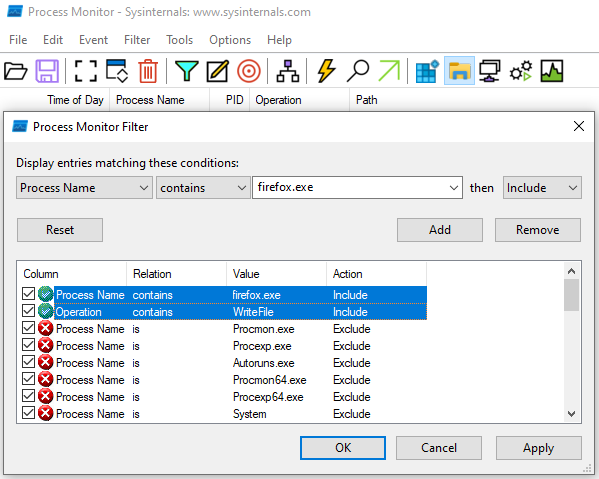
\includegraphics{bilder/process-monitor-filter.png}}}
%	\label{...}
	\caption{Tabelle mit wiederherstellbaren Dateien: Logfile 1 vs. Logfile 2}
\end{figure}
Wie in Abbildung X dargestellt werden dazu ausschließlich die Option "File System Activity" ausgewählt.
Anschließend wird als Prozessname der Browserprozess gesetzt:
\begin{itemize}
\item[\textbf{Firefox}] firefox.exe
\item[\textbf{Tor-Browser}] firefox.exe und tor.exe
\item[\textbf{Chrome}] chrome.exe
\item[\textbf{Brave}] brave.exe
\end{itemize}
Weiterhin wird als Prozessoperation "WriteFile" gesetzt, um ausschließlich Schreibaktivitäten zu filtern. Hintergrund ist, dass PB Artefakte nur über "WriteFile" Operationen entstehen können, nicht über beispielsweise Löschoperationen.

Daraufhin wird die gefilterte Logfile als CSV exportiert, um sie dann in Excel zu öffnen und irrelevante Spalten sowie Duplikate zu löschen.
Abschließend werden alle geschriebenen Dateien nach nach browserspezifischen Speicherorten gruppiert.

\paragraph*{Prüfung auf PB Artefakte}
Nachdem die geschriebenen Browserdateien identifiziert und kategorisiert wurden, wird für jede Datei geprüft, ob PB Artefakte enthalten sind. Die zur Dateiextraktion sowie Dateianalyse notwendigen Schritte sind in Abbildung X (TODO!) dargestellt.
\begin{figure}[h!]
	\centering
	\small
	\centerline{\resizebox{\linewidth}{!}{\input{bilder/process_monitor_to_exce-Latexl.pdf_tex}}}
	\caption{TODO: Process Monitor Write Operation to Excel Spreadsheet}
	\label{fig:jes}
\end{figure}

Zur Dateiextraktion sind werden folgende Schritte durchgeführt.
\begin{enumerate}
\item In Autopsy prüfen, ob Datei in Festplatten-Image des entsprechenden VM-Snapshots vorhanden ist. Welcher Snapshot bei welchem Logfile untersucht wird ergibt sich aus dem Browsing Szenario in Kapitel X. 
\item Wenn ja, Datei mit Autopsy extrahieren.
\item Wenn nein, prüfen, ob Datei in Arbeitsspeicher vorhanden. Dazu wird überprüft, ob die Datei in der Ausgabe des Volatiltiy Plugins "filescan" (\texttt{vol.py -f ram\_dump.img windows.filescan > filescan.txt}) vorhanden ist. Welcher RAM-Dump bei welchem Logfile untersucht wird, ergibt sich aus dem Browsing Szenario in Kapitel X.
Wenn eine Datei in der Ausgabe gefunden wurde, wird sie mithilfe des Volatility "dumpfiles"  Plugins anhand ihrer virtuellen Dateispeicheradresse extrahiert. (TODO: Befehl)
Die Abhängigkeit zwischen den beiden Plugins ist in Abbildung X dargestellt.
%\begin{figure}[h!]
%	\centering
%	\small
%	\centerline{\resizebox{0.8\linewidth}{!}{\input{bilder/volatility-filescan-dumpfiles-Latex.pdf_tex}}}
%	\caption{Datensammlung Zeitpunkte Tor}
%	\label{fig:jes}
%\end{figure}
\item Wenn Datei auch nicht im RAM vorhanden ist: Prüfen, ob es um eine temporäre Datei (meistens Endung ".tmp") handelt.
\item Wenn es sich um eine temporäre Datei handelt, wird die entsprechende Nicht-temporäre gewählt und und erneut bei Schritt 1 begonnen. Wenn beispielsweise die Datei "some-file.json.tmp" nicht existiert wird geprüft prüfen, ob die Datei "some-file.json" existiert.
\item Wenn es sich um keine temporäre Datei handelt: Datei als "nicht wiederherstellbar"  markieren
\end{enumerate}

Nachdem eine Datei extrahiert werden konnte, werden folgende Schritte zur Dateianalsye durchgeführt.
\begin{enumerate}
	\setcounter{enumi}{7}
	\item Datei mit entsprechdem Tool untersuchen 
	\item Wenn Datei nicht lesbar ist: Datei mir zusätzlichem Tool vorverarbeiten. Beispielsweise werden komprimierte Dateien dekomprimiert. 
	\item In Excel-Tabelle markieren, ob die Datei private Browsing Artefakte enthält. Dabei gibt es drei Zustände: 
	\begin{itemize}
	\item leere Datei
	\item neuer (nicht-leerer) Inhalt
	\item gleichbleibender Inhalt
	\end{itemize}		
\end{enumerate}


\subsubsection*{SQLite-Datenbänke}

Eine besondere Rolle unter den Common Locations bei Browsern nehmen SQLite Datenbänke ein. 
Sie ermöglichen Browsern das Speichern und Verwalten von Nutzerinformationen, wie Lesezeichen, Browserverlauf, Caches, Cookies in Datenbankdateien zu speichern, ohne einen separaten Datenbankserver zu benötigen.

\begin{figure}[h!]
	\centering
	\small
	\centerline{\resizebox{\linewidth}{!}{\input{bilder/sqlite-methodology-Latex.pdf_tex}}}
	\caption{TODO: Process Monitor Write Operation to Excel Spreadsheet}
	\label{fig:jes}
\end{figure}
Wie in Abbildung X dategestellt erfolgt die Dateiextraktion analog zur Vorgehensweise bei den Schreiboperationen der Process Monitor Logfiles.

Um die SQLite Datenbänke zu analysieren wird jede Datenbank mit der gleichen Datenbank aus dem vorherigem Snapshot mithilfe des Befehlszeilentools "sqldiff.exe" (\texttt{sqldiff.exe database1.sqlite database2.sqlite}) verglichen. Die Inhaltsunterschiede werden für jede Datei in jedem Snapshot untersucht und in einer Excel Tabelle festgehalten.

Für jede SQLite Datenbank gibt es einen "Write-Ahead Log", kurz WAL. In dieser Datei werden Datenbankänderungen vorübergehend protokolliert, bevor sie dauerhaft in die Hauptdatenbankdatei geschrieben werden. 
Um potentielle PB Artefakte im WAL zu berücksichtigen, wird der WAL mithilfe der sqlite3 Befehlszeile (\texttt{sqlite3> PRAGMA wal\_checkpoint;}) in die SQLite-Datei geschrieben.

\subsection{Uncommon Locations}
Ungewöhnliche Speicherorte beziehen sich auf Verzeichnisse, die nicht zu den gängigen Speicherorten gehören. 
Bei Festplatten-Images handelt es sich dabei meist um Dateien des Betriebssystems oder andere Festplattenbereiche, wie beispielsweise unallokierte Speicherbereiche oder der Arbeitsspeicher.

Uncommon Locations werden ohne Vorwissen über das Browserverhalten sowie ohne Vorverarbeitung der Dateien mithilfe der "Blackbox-Analyse" untersucht \cite{Bonetti.2014}:
Im Kontext der Browser Forensik werden dazu Stringsuchen nach PB Artefakten über die gesamten Speicherabbilder durchgeführt.
Dies ist nur durch Unterstützung mit Forensik-Tools möglich. Somit wird bei der Analyse der Uncommon Locations in die Vollständigkeit der Tools vertraut.

\subsubsection*{Analyse mit Autopsy}
Bei den Uncommon Locations wird Autopsy als forensisches Werkzeug zur Analyse der Festplatten-Images verwendet.
Dazu wird eine Stichwortsuche mit den in Tabelle X definierten PB Artefakten über das gesamte eingelesene Festplatten-Image durchgeführt.

Autopsy bietet dazu die in Abbildung X dargestellte Funktion an, zur Suche nach Strings, Teilstrings oder regulären Ausdrücken in Dateinamen und Dateiinhalten.
\begin{figure}[h!]
	\resizebox{0.85\linewidth}{!}{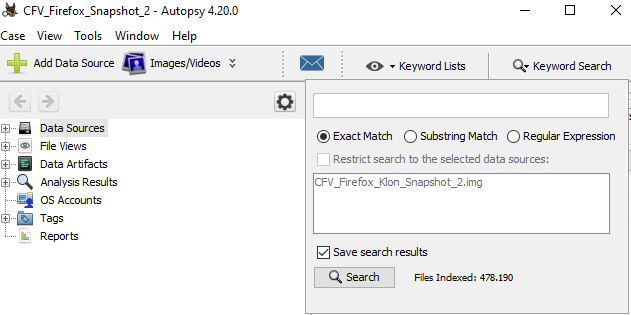
\includegraphics{bilder/autopsy-search.png}}
%	\label{...}
	\caption{Tabelle mit wiederherstellbaren Dateien: Logfile 1 vs. Logfile 2}
\end{figure}

Zusätzlich kategorisiert Autopsy beim Einlesen eines Festplatten-Images automatisch die Dateien. Für diesen Versuch sind folgende Dateikategorien von Interesse:
\begin{itemize}
\item Web Bookmarks
\item Web Cookies
\item Web History
\item Web Categories
\end{itemize}


\subsubsection*{Analyse mit Volatility}
Bei der Analyse des Arbeitsspeichers als Uncommon Location ist es kritisch, dass ein gefundener String eindeutig einem Browserprozess zugeordnet werden kann. 

In der Literatur wird der Arbeitsspeicher oft unzureichend analysiert, indem eine Stringsuche im RAM-Dump durchgeführt ist, der als Binärdatei in einem Hexadezimaleditor geöffnet ist. \cite{Rochmadi.2017, Md.2018, Montasari.2015}
Wie in Abbildung X und Y gezeigt, wird ein String, der in einer Textdatei auf dem Desktop gespeichert ist ebenfalls im Hexadezimaleditor HxD angezeigt, obwohl kein Browsing Szenario durchgeführt wurde.
\begin{figure}[h!]
	\centerline{\resizebox{0.5\linewidth}{!}{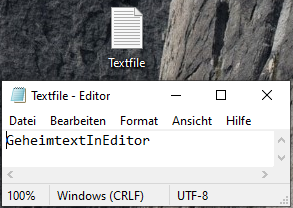
\includegraphics{bilder/ram-editor1.png}}}
%	\label{...}
	\caption{Tabelle mit wiederherstellbaren Dateien: Logfile 1 vs. Logfile 2}
\end{figure}
\begin{figure}[h!]
	\resizebox{\linewidth}{!}{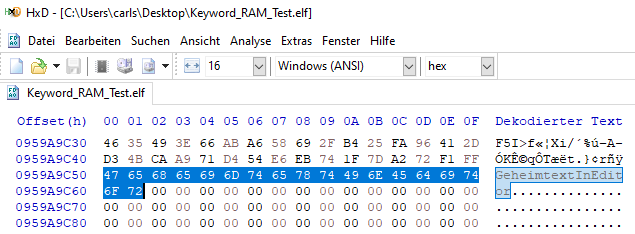
\includegraphics{bilder/ram-editor2.png}}
%	\label{...}
	\caption{Tabelle mit wiederherstellbaren Dateien: Logfile 1 vs. Logfile 2}
\end{figure}

Um einen im RAM gefundenen String einem Browserprozess zuordnen zu können, wird deshalb das forensiche Analysetool Volatility mit dem PlugIn "Yarascan" verwendet.

YARA ist ein flexibles Tool, um mithilfe sogenannter "YARA-Regeln" nach bestimmten Mustern im Arbeitsspeicher zu suchen.
Die für diesen Versuch verwendeten Yara-Regeln entsprechen den Strings der PB Artefakte in Tabelle X in Kapitel Y. Zusätzlich sucht eine Regel nach HTML-Fragmenten, die eindeutig einer besuchten Seite des Browsing-Szenarios zuzuordnen sind. \cite{Said.2011}
Alle verwendeten Yara-Regeln sind im Anhang X (TODO!) aufgelistet.

Um den RAM-Dump nach den Yara-Regeln zu durchsuchen wird folgender Befehl ausgeführt: \texttt{vol.py -f ram\_dump.img windows.vadyarascan --yara-file yara\_rules.yara > yarascan.txt}
Nachdem der RAM-Dump nach den Regeln durchsucht wurde, gibt die Yarascan-Ausgabe für jeden gefundenen String die PID des Prozesses, in dem der String gefunden wurde sowie die virtuelle Speicheradresse des gefundenen Strings an.

\begin{figure}[h!]
	\centering
	\small
	\centerline{\resizebox{\linewidth}{!}{\input{bilder/yarascan_plugin_tree-Latex.pdf_tex}}}
	\caption{TODO: Process Monitor Write Operation to Excel Spreadsheet}
	\label{fig:jes}
\end{figure}
Wie in Abbildung X dargestellt, wird davon ausgehend mit dem Plugin "pslist" (\texttt{vol.py -f ram\_dump.img windows.pslist --pid <PID> > pslist.txt}) der Prozessname der PID ermittelt, in dem der String gefunden wurde.

Oft ist für bei einem gefundenen String von Interesse, ob in den Speicheradressen vor und nach dem Treffer weitere Zusammenhänge erkennbar sind.
Mithilfe des Plugins "memmap" (\texttt{vol.py -f ram\_dump.img windows.memmap --pid <PID> > memmap.txt}) wird die Abbildung der virtuellen Speicheradressen eines Prozesses auf die Byte-Offset der extrahierten Speicherseite des Prozesses ermittelt.
Diese Seite kann mithilfe des "--dump" Flags extrahiert werden: \texttt{vol.py -f ram\_dump.img -o $\backslash$dump\_dir$\backslash$ windows.memmap --pid <PID> --dump}
In einem Hexadezimaleditor, wie HxD, kann der String-Treffer anhand des ermittelten Byte-Offsets in der Speicherseite gefunden werden.

\subsection{Registry}
Die letzte Kategorie analysierter Daten umfasst die Artefakte der Registry.
Diese zählen sowohl zu den Common als auch Uncommon Locations und werden deshalb eigene Kategorie aufgeführt.

\paragraph*{Common Locations}

*** TODO: Common location: Shellactivities Key ***
	existiert nicht mehr --> Nicht mehr vorhanden in aktueller Version (Verweis auf E-Mail)

Als Teil der Common Locations werden die Registry-Aktivitäten in den Process Monitor Logfiles analysiert.
Dazu wird jede Logfile in Process Monitor eingelesen und wie in Abbildung X gezeigt gefiltert.
\begin{figure}[h!]
	\centerline{\resizebox{0.7\linewidth}{!}{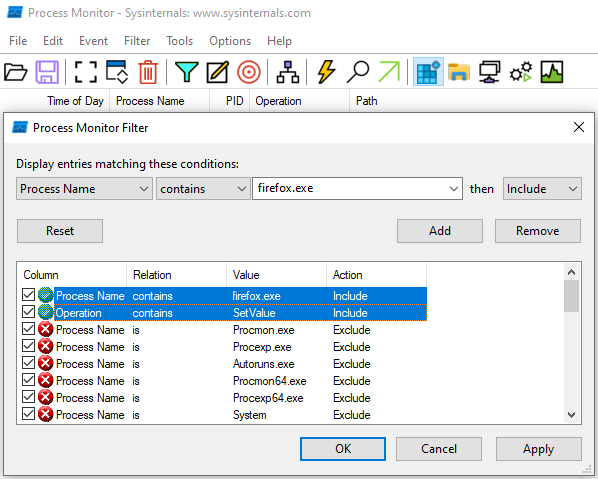
\includegraphics{bilder/process-monitor-filter-registry.png}}}
%	\label{...}
	\caption{Tabelle mit wiederherstellbaren Dateien: Logfile 1 vs. Logfile 2}
\end{figure}
Zunächst wird ausschließlich die Option "Registry Activity" ausgewählt.
Anschließend wird nach Browser-Prozessnamen analog zu den Schreiboperationen in Kapitel X gefiltert.
Das gefilterte Logfile wird als CSV Datei exportiert und in Excel weiter verarbeitet.
Zunächst werden gleiche Schreiboperationen gelöscht.
Anschließend werden die geschriebenen Registry Keys browserspezifisch gruppiert.
	
\paragraph*{Uncommon Locations}
Als Uncommon Location werden alle Registry Hives in jedem Festplatten-Image mit dem "Registry Explorer" untersucht.
Jedes Hive hat eine bestimmte Funktion, wie die Speicherung von Systemeinstellungen (System-Hives) oder individuellen Benutzerkonfigurationen (User-Hives). Diese in Tabelle X dargestellten Hives werden von Windows beim Start geladen und dienen als Quelle für Einstellungen und Informationen, die von verschiedenen Systemkomponenten und Anwendungen genutzt werden.	
 % https://medium.com/@haircutfish/tryhackme-windows-forensics-1-task-3-accessing-registry-hives-offline-task-4-data-acquisition-b440f5be2a13
Zur Analyse wird jeder Hive aus einem VM-Snapshot extrahiert und in eine Registry Explorer Sitzung geladen, anschließend wird eine Stringsuche nach PB Artefakten in allen geladenen Hives gleichzeitig durchgeführt.

\begin{table}[h!]
%\resizebox{\linewidth}{!}{
\begin{tabular}{lllll}
\cline{1-2}
\multicolumn{2}{|c|}{\textbf{System-Hives (C:\textbackslash{}\textbackslash{}Windows\textbackslash{}\textbackslash{}System32\textbackslash{}\textbackslash{}Config)}} &  &  &  \\ \cline{1-2}
\multicolumn{1}{|l|}{\textbf{Dateiname}}             & \multicolumn{1}{l|}{\textbf{Inhalt}}                                                                           &  &  &  \\ \cline{1-2}
\multicolumn{1}{|l|}{\textit{DEFAULT}}               & \multicolumn{1}{l|}{Standardkonfigurationseinstellungen für neue Benutzerprofile.}                             &  &  &  \\ \cline{1-2}
\multicolumn{1}{|l|}{\textit{SAM}}                   & \multicolumn{1}{l|}{Sicherheitskontensdaten, einschließlich der Benutzerkonten und deren Kennwörter.}          &  &  &  \\ \cline{1-2}
\multicolumn{1}{|l|}{\textit{SECURITY}}              & \multicolumn{1}{l|}{Sicherheitsinformationen für die Zugriffssteuerung und Authentifizierung.}                 &  &  &  \\ \cline{1-2}
\multicolumn{1}{|l|}{\textit{SOFTWARE}}              & \multicolumn{1}{l|}{Konfigurationsdaten für installierte Software und Anwendungen.}                            &  &  &  \\ \cline{1-2}
\multicolumn{1}{|l|}{\textit{SYSTEM}}                & \multicolumn{1}{l|}{Systemkonfigurationseinstellungen und Gerätetreiberinformationen.}                         &  &  &  \\ \cline{1-2}
                                                     &                                                                                                                &  &  &  \\ \cline{1-2}
\multicolumn{2}{|c|}{\textbf{User-Hives (C:\textbackslash{}\textbackslash{}Users\textbackslash{}\textbackslash{}\textless{}username\textgreater{})}}                  &  &  &  \\ \cline{1-2}
\multicolumn{1}{|l|}{\textbf{Dateiname}}             & \multicolumn{1}{l|}{\textbf{Inhalt}}                                                                           &  &  &  \\ \cline{1-2}
\multicolumn{1}{|l|}{\textit{NTUSER.DAT}}            & \multicolumn{1}{l|}{Individuelle Einstellungen und Konfigurationen für den angemeldeten Benutzer}              &  &  &  \\ \cline{1-2}
\multicolumn{1}{|l|}{\textit{USRCLASS.DAT}}          & \multicolumn{1}{l|}{Dateizuordnungen und Registrierungseinstellungen für den angemeldeten Benutzer}            &  &  &  \\ \cline{1-2}
\end{tabular}
%}
\end{table}
	

